% class
\documentclass[a4paper,12pt,xelatex,ja=standard]{bxjsarticle}

% packages
%% mathematical notations
\usepackage{amsthm,amsmath,amssymb,amsfonts} % mathematical notations
\usepackage{bm} % bold character
\usepackage{latexsym} % more mathematical notations
\usepackage{physics} % physical notations
\usepackage{mathtools} % math tools
%% graphs
\usepackage{graphicx, xcolor} % graph
\usepackage{circuitikz} % for circuit elements
\usepackage{float} % positioning of graphs
\usepackage{siunitx} % SI units
\usepackage{tikz} % graphic elements
\usepackage{wrapfig} % must be after float package.
\usepackage{askmaps} % Karnaugh map
%% type system
\usepackage{bussproofs} % proof tree
%% code
\usepackage[ruled,vlined]{algorithm2e} % pseudo code
\usepackage{listings} % source code
\usepackage{inconsolata}
\lstset{
  basicstyle=\footnotesize,
  numbers=left,
  frame={tb}
}
\usetikzlibrary{automata, positioning, calc, quotes}
\tikzset{
  ->,
  >={Stealth[round]},
  auto,
  every state/.style={draw},
  node distance=3cm
}
\newcommand\DoubleLine[5][4pt]{%
    \path(#2)--(#3)coordinate[at start](h1)coordinate[at end](h2);
    \draw[<-,very thick,black] ($(h1)!#1!90:(h2)$)  to ["#4"]   ($(h2)!#1!-90:(h1)$);
    \draw[->,very thick,  red] ($(h1)!#1!-90:(h2)$) to ["#5" '] ($(h2)!#1!90:(h1)$);
    }

% Basic information
\title{電子情報学専攻 \, 専門 \\ 平成29年 \, 解答・解説}
\author{diohabara}
\date{\today}

\begin{document}
\maketitle

\section*{第1問\ 電気・電子回路}

\section*{第2問\ 論理回路}
\subsection*{(1)}
求める最も状態数の少ない状態遷移図は次の通り。
\begin{center}
  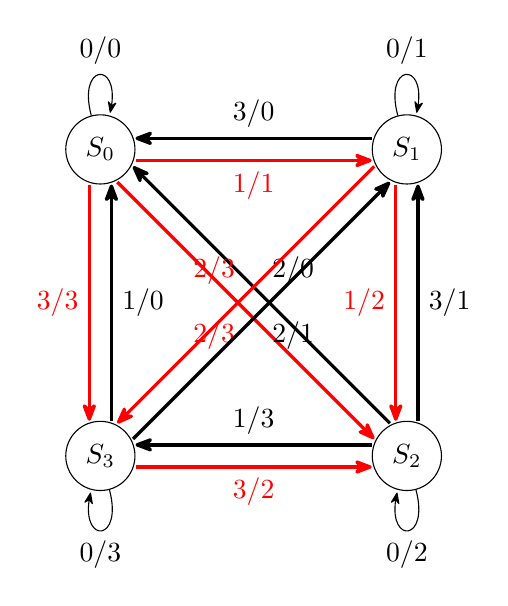
\begin{tikzpicture}
    \node[state] (ul) {$S_0$};
    \node[state] (ur) [right =of ul]{$S_1$};
    \node[state] (lr) [below =of ur]{$S_2$};
    \node[state] (ll) [below =of ul]{$S_3$};

    \DoubleLine{ul}{ur}{3/0}{1/1}
    \DoubleLine{ul}{lr}{2/0}{2/3}
    \DoubleLine{ul}{ll}{1/0}{3/3}
    \DoubleLine{ur}{lr}{3/1}{1/2}
    \DoubleLine{ur}{ll}{2/1}{2/3}
    \DoubleLine{ll}{lr}{1/3}{3/2}

    \path
      (ul)
        edge [loop above] node {0/0} (ul)
      (ur)
        edge [loop above] node {0/1} (ur)
      (lr)
        edge [loop below] node {0/2} (lr)
      (ll)
        edge [loop below] node {0/3} (ll)
    ;
  \end{tikzpicture}
\end{center}

\subsection*{(2)}
\begin{table}[H]
  \centering
  \begin{tabular}{|l|l|l|l||l|l|}
  \hline
  $I_1$ & $I_0$ & $S_1$ & $S_0$ & $S_1'$ & $S_0'$ \\ \hline \hline
  0     & 0     & 0     & 0     & 0      & 0      \\ \hline
  0     & 0     & 0     & 1     & 0      & 1      \\ \hline
  0     & 0     & 1     & 1     & 1      & 1      \\ \hline
  0     & 0     & 1     & 0     & 1      & 0      \\ \hline
  0     & 1     & 1     & 0     & 1      & 1      \\ \hline
  0     & 1     & 1     & 1     & 0      & 0      \\ \hline
  0     & 1     & 0     & 1     & 1      & 0      \\ \hline
  0     & 1     & 0     & 0     & 0      & 1      \\ \hline
  1     & 1     & 0     & 0     & 1      & 1      \\ \hline
  1     & 1     & 0     & 1     & 0      & 0      \\ \hline
  1     & 1     & 1     & 1     & 1      & 0      \\ \hline
  1     & 1     & 1     & 0     & 0      & 1      \\ \hline
  1     & 0     & 1     & 0     & 0      & 0      \\ \hline
  1     & 0     & 1     & 1     & 0      & 1      \\ \hline
  1     & 0     & 0     & 1     & 1      & 1      \\ \hline
  1     & 0     & 0     & 0     & 1      & 0      \\ \hline
  \end{tabular}
\end{table}

\subsection*{(3)}
カルノー図は次の通り。

\begin{figure}[H]
  \centering
  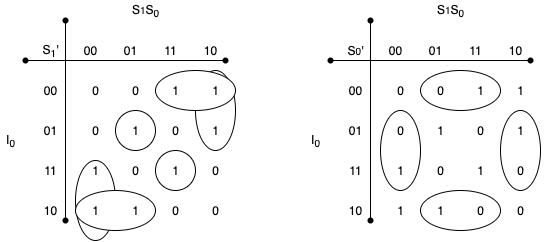
\includegraphics[width=11cm]{images/2018_karnaugh.png}
\end{figure}

よって加法標準形は
\begin{equation*}
  \begin{split}
    S_1'
      &= I_1 \overline{S_1} \overline{S_0} + I_1 \overline{I_0} \overline{S_1} + \overline{I_1} \overline{I_0} S_1 + \overline{I_1} S_0 \overline{S_0} + \overline{I_1}I_0 \overline{S_1}S_0 + I_1 I_0 S_1 S_0 \\
    S_0'
      &= \overline{I_0}S_0 + I_0 \overline{S_0}
  \end{split}
\end{equation*}

\subsection*{(4)}
求める回路は次の通り。
TODO
% \begin{figure}[H]
%   \centering
%   \includegraphics[width=11cm]{images/2018_4_circuit.png}
% \end{figure}

\section*{第3問\ アルゴリズムとデータ構造}
\subsection*{(1)}
GDFEA

\subsection*{(2)}
B, C, A, E, F, D, G

\subsection*{(3)}
ソフトウェアの依存関係の解決。\\
ソフトAをインストールした後でないとソフトBをインストールできないなど、インストールをする順番がある場合、この依存関係を有向グラフで表し、トポロジカルソートを求めることで依存関係を解決してインストールができる。

\subsection*{(4)}
\begin{lstlisting}[caption=DFSの擬似コード]
function DFS(Vertex u)
  visited[u] = TRUE
  foreach v in Adj[u]
    if visited[v] != TRUE
      DFS(v)
  s.push(u)
\end{lstlisting}

\subsection*{(5)}
$|V|$の頂点それぞれについて1度だけDFSが呼び出され、$|E|$の辺がそれぞれ1度ずつ参照されるので求める時間計算量は$O(|V| + |E|)$となる。

\subsection*{(6)}
\subsubsection*{アルゴリズム}
各頂点の入次数を表す配列degreeと、入次数が0の頂点集合を保持するキューQと、トポロジカルソートの順に頂点を格納するキューSを用意する。まず、すべての頂点について、入ってくる辺の本数を数えdegreeに記録して、degree[v] = 0であるような頂点vをすべてQにpushする。そして、Qが空になるまで以下の操作を繰り返す。
\begin{itemize}
  \item Qから頂点uを取り出し、Sにpushする
  \item 頂点uから出ているすべての辺(u, v)について、degree[v]を1減らす。このとき、degree[v]が0となった場合は、頂点vをQにpushする
\end{itemize}
この操作が終了したとき、Sに頂点を追加した順番がトポロジカルソートとなっている。

\subsubsection*{時間計算量}
辺を参照する回数はdegreeの前計算の際に$|E|$回と操作1~2の際に$|E|$で合わせて$2|E|$回。Qへのpush・popの回数とSへのpushの回数はそれぞれ$|V|$回なので、このアルゴリズムの時間計算量は$O(|V| + |E|)$となる。

\section*{第4問\ ネットワーク}

\section*{第5問\ 信号処理}
\subsection*{(1)}
片側Z変換の定義は
\[
  X(z) = \sum^{\infty}_{n=0}x(n)z^{-n}
\]

\subsection*{(2)}
抵抗部分のインピーダンスはR、キャパシタ部分のインピーダンスは$\frac{1}{j\omega C}=\frac{1}{sC}$となるので、

\begin{equation*}
  \begin{split}
    &V_{out}(s) = \frac{\frac{1}{sC}}{R + \frac{1}{sC}}V_{in}(s)\\
    &H(s) = \frac{V_{out}(s)}{V_{in}(s)} = \frac{1}{1 + sRC} = \frac{1}{1 + s}
  \end{split}
\end{equation*}

と求められる。

\subsection*{(3)}
$z=e^{sT}$から導出したい式は
\begin{equation*}
  s \approx \frac{2}{T} \frac{1 - z^{-1}}{1 + z^{-1}}
\end{equation*}
これを直接導こうとすると大変なので、これをzについて解いた形に変形する。

\begin{equation*}
  \begin{split}
    &\frac{sT}{2} \approx \frac{1 - z^{-1}}{1 + z^{-}} \\
    &1 + \frac{sT}{2} \approx \frac{2}{1 + z^{-1}} \\
    &1 - \frac{sT}{2} \approx \frac{2z^{-1}}{1 + z^{-1}}\\
    &\frac{1 - \frac{sT}{2}}{1 + \frac{sT}{2}} \approx z^{-1} = e^{sT}
  \end{split}
\end{equation*}

すると一番下の式は

\begin{equation*}
  e^{-sT} = \frac{e^{-\frac{sT}{2}}}{e^{\frac{sT}{2}}}
\end{equation*}

と近似すれば導出が可能なので、これを下から上にたどっていけば求める近似式の導出が可能。

\subsection*{(4)}
$H(s) = \frac{1}{1+s}$に$s = \frac{2}{T}\frac{1 - z^{-1}}{ 1 + z^{-1}} = 2 \frac{1 - z^{-1}}{1 + z^{-1}}$を代入すると

\begin{equation*}
  \begin{split}
    H(z)
      &= \frac{1}{1 + 2 \frac{1 - z^{-1}}{1 + z^{-1}}} \\
      &= \frac{1 + z^{-1}}{3 - z^{-1}}
  \end{split}
\end{equation*}

と求められる。

\subsection*{(5)}
入力を$X(z)$、出力を$Y(z)$として方程式を立てると

\begin{equation*}
  \begin{split}
    &H(z) = \frac{Y(z)}{X(z)} = \frac{1 + z^{-1}}{3 - z^{-1}} \\
    &(3 - z^{-1}) Y(z) = (1 + z^{-1})X(z) \\
    &Y(z) = \frac{1}{3}(X(z) + z^{-1}(X(z) + Y(z)))
  \end{split}
\end{equation*}

あとはこれをもとに回路を組めばよく以下の通り。

\begin{figure}[H]
  \centering
  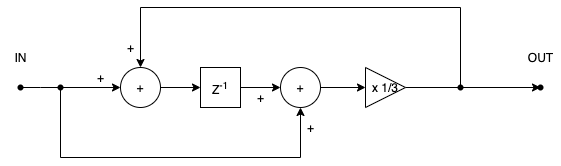
\includegraphics[width=11cm]{images/2018_5_circuit.png}
\end{figure}

\subsection*{(6)}
(2)と同様にこの回路におけるH(s)を求める。
\begin{equation*}
  \begin{split}
    &V_{out}(s) = \frac{R}{R + \frac{1}{sC}}V_{in}(s) \\
    &H(s) = \frac{V_{out}(s)}{V_{in}(s)} = \frac{sRC}{1 + sRC} = \frac{s}{1 + s}
  \end{split}
\end{equation*}

(4)と同様に$s = 2 \frac{1 - z^{-1}}{1 + z^{-1}}$を代入すると

\begin{equation*}
  \begin{split}
    H(z)
      &= \frac{2 \frac{1 - z^{-1}}{1 + z^{-1}}}{1 + 2 \frac{1 - z^{-1}}{1 + z^{-1}}} \\
      &= 2 \frac{1 - z^{-1}}{3 - z^{-1}}
  \end{split}
\end{equation*}

(5)と同様に$X(z)$、$Y(z)$の方程式で書き直す。

\begin{equation*}
  \begin{split}
    H(z) &= \frac{Y(z)}{X(z)} = 2 \frac{1 - z^{-1}}{3 - z^{-1}}\\
    (3-z^{-1})Y(z) &= 2 (1 - z^{-1})X(z) \\
    Y(z) &= \frac{1}{3}(2 X(z) + z^{-1}(-2 X(z) + Y(z)))
  \end{split}
\end{equation*}

よって、この場合も方程式をもとに回路を組めば良いので以下の通り。

\begin{figure}[H]
  \centering
  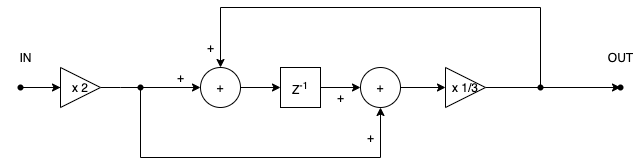
\includegraphics[width=11cm]{images/2018_6_circuit.png}
\end{figure}

\end{document}
